\documentclass[10pt]{scrartcl}
\usepackage[mdthm,colorsec,noauthor,noasy]{evan}
\usepackage{handout}
\usepackage[T1]{fontenc}
\usepackage{lmodern}
\usepackage{listings}
\lstset{language=Python,emptylines=1,basicstyle=\ttfamily\normalsize,identifierstyle=\color{black},keywordstyle=\color{NavyBlue},commentstyle=\color{black!60},stringstyle=\color{RawSienna},showstringspaces=false,columns=fullflexible,keepspaces=true,upquote=true,aboveskip=5pt,belowskip=5pt}
\newcommand{\py}[1]{\texttt{#1}}
\newcommand{\hint}[1]{\par\emph{Hint:} #1\par}
\newcommand{\codeblock}[1]{\par\noindent\begin{minipage}{\linewidth}\csname code#1\endcsname\end{minipage}\par}
\expandafter\def\csname codeteamwork\endcsname{\lstinputlisting[firstline=4,lastline=13]{discussion_solutions.py}}
\expandafter\def\csname codekeeper\endcsname{\lstinputlisting[firstline=17,lastline=24]{discussion_solutions.py}}
\expandafter\def\csname codefind_digit\endcsname{\lstinputlisting[firstline=28,lastline=30]{discussion_solutions.py}}
\expandafter\def\csname codematch_k\endcsname{\lstinputlisting[firstline=34,lastline=41]{discussion_solutions.py}}
\expandafter\def\csname codewhich\endcsname{\lstinputlisting[firstline=45,lastline=53]{discussion_solutions.py}}
\expandafter\def\csname codeevery\endcsname{\lstinputlisting[firstline=57,lastline=65]{discussion_solutions.py}}
\expandafter\def\csname codecount_if\endcsname{\lstinputlisting[firstline=69,lastline=80]{discussion_solutions.py}}
\expandafter\def\csname codenew_print\endcsname{\lstinputlisting[firstline=4,lastline=10]{exam_solutions.py}}
\expandafter\def\csname codegap_tool\endcsname{\lstinputlisting[firstline=14,lastline=19]{exam_solutions.py}}
\expandafter\def\csname codemake_gap\endcsname{\lstinputlisting[firstline=23,lastline=35]{exam_solutions.py}}
\expandafter\def\csname codefunsquare\endcsname{\lstinputlisting[firstline=39,lastline=59]{exam_solutions.py}}
\expandafter\def\csname codesummation\endcsname{\lstinputlisting[firstline=4,lastline=9]{examples.py}}
\expandafter\def\csname codetwice\endcsname{\lstinputlisting[firstline=13,lastline=19]{examples.py}}
\expandafter\def\csname coderetained\endcsname{\lstinputlisting[firstline=23,lastline=32]{examples.py}}
\expandafter\def\csname codecurry\endcsname{\lstinputlisting[firstline=36,lastline=41]{examples.py}}
\expandafter\def\csname codenearest\endcsname{\lstinputlisting[firstline=56,lastline=64]{examples.py}}
\expandafter\def\csname codepiecewise\endcsname{\lstinputlisting[firstline=4,lastline=7]{lab_solutions.py}}
\expandafter\def\csname codecount_cond\endcsname{\lstinputlisting[firstline=11,lastline=19]{lab_solutions.py}}
\expandafter\def\csname codecycle\endcsname{\lstinputlisting[firstline=23,lastline=37]{lab_solutions.py}}
\expandafter\def\csname codelab_diagram\endcsname{\lstinputlisting[firstline=41,lastline=57]{lab_solutions.py}}

\title{CS 61A --- Week 3}
\subtitle{September 7--13: Abstraction and Function Examples\\Lectures 6--7; Lab 2; Discussion 2}
\author{}\date{}\ihead{}
\begin{document}\maketitle
\section{Delay a computation until its input is known}
\begin{qbox}
How can the same summation loop add $1+2+3+4+5$ or $1/2+1/4+1/8+1/16+1/32$? What does \py{lambda x: pow(1/2,x)} produce before any number is supplied?
\end{qbox}
A \textbf{higher-order function} accepts a function, returns a function, or both. Functions are values: \py{f} is a function value; \py{f(x)} calls that value and may return a number, another function, or \py{None}. The distinction determines what the next pair of parentheses can do.
\begin{proposition*}[Lambda creation and application --- Lecture 6, slides 3--8,12; Lab 2 review]
Evaluating \py{lambda parameters: expression} creates a function whose parent is the current frame. It does not execute the body or bind a name. A later call binds arguments in a new local frame and returns the body's expression value. The body is one expression; it cannot contain an assignment or a \py{while} statement. There may be zero, one, or several parameters.
\end{proposition*}
\begin{motive}
\ii[Want.] Supply a rule for the next term without computing it before the loop knows its index.
\ii[Know.] A function can accept the index later. Its body runs only when called.
\ii[Key step.] Pass the function itself as \py{term}; call \py{term(k)} inside the unchanged loop. A lambda writes this small rule directly where it is needed.
\end{motive}
\codeblock{summation}
The unused \py{common\_ratio} assignment is deliberately retained from Lecture 6's environment example; it is local to this call. Before each test, \py{total} is the sum of terms 1 through \py{k-1}. Adding the next term and increasing \py{k} preserves that statement; at \py{k=n+1} the result is the requested sum.
\begin{example*}[Actual Lecture 6 summations]
\py{summation(5, lambda x: x)} gives $1+2+3+4+5=15$.
\py{summation(5, lambda x: pow(1/2,x))} gives $(16+8+4+2+1)/32=31/32$.
The named alternatives \py{identity(k)=k}, \py{cube(k)=pow(k,3)}, and \py{pi\_term(k)=8/(4*k-3)/(4*k-1)} supply the same one-argument interface. For cubes the result is $1+8+27+64+125=225$; for the first five pi terms it is approximately $3.041839618929402$.
\end{example*}
Assignment \py{term = lambda x: pow(1/2,x)} both creates a function and binds it. The equivalent \py{def term(x): return pow(1/2,x)} creates a named function and binds it. A bare lambda expression creates no binding. In diagrams label its function value $\lambda$ and its source line; Python's runtime name is \py{<lambda>}.

\method{Rewrite nested lambdas one function at a time.}
\py{(lambda f: lambda x: f(f(x)))(lambda y: y*y)(3)} first supplies the square function, then supplies $3$. It computes $3\to9\to81$. The corresponding definitions are:
\codeblock{twice}
\py{twice(square)(3)} gives $81$. The call \py{twice(square)} returns \py{g}; it does not call \py{square} yet. Every lambda can be replaced by a definition at its creation site with the same parameters, return expression and defining environment. Use a fresh name for each replacement definition so it does not replace an existing binding. A multi-statement function body cannot be copied directly into a single lambda body.

\method{Choose a value with a conditional expression --- Lecture 7.}
\py{a if condition else b} evaluates the condition first, then only the selected branch. For example, \py{1 if True else 1/0} returns $1$. This lets Lab 2's piecewise function return \py{f(x) if x < b else g(x)}. In contrast, both operands of an ordinary two-argument call are evaluated before its body runs.
\begin{shortcuts}
\ii For a chained call, evaluate its operator first: \py{multiply\_by(3)(10)} first creates a function retaining $3$, then calls it on $10$, returning $30$. Naming it \py{times\_three} gives \py{times\_three(5)=15}; its inner name need not exist globally.
\ii Lab 2's \py{scale(f,x,k)=k*f(x)} gives \py{scale(square,3,2)=18}, \py{scale(square,2,5)=20}, and \py{scale(lambda x:x+10,5,2)=30}. Bind \py{f} to the supplied function before tracing its call.
\ii Lecture 7's \py{f=abs; x=-3; f(f(x))} gives $3$. Its lambda version \py{h=lambda f:lambda x:f(f(x)); h(abs)(-3)} also gives $3$.
\end{shortcuts}
\begin{trapbox}
\ii Returning \py{f(f)} supplies a function as \py{f}'s argument; it does not mean ``apply twice to a later input.'' For \py{f=lambda x:3*x}, it raises \py{TypeError}.
\ii Defining \py{print\_lambda=lambda z:print(z)} prints nothing. Calling \py{print\_lambda(1000)} prints $1000$ and returns \py{None}. A zero-argument function such as a die likewise still needs \py{()} to execute.
\ii \py{a and b} and \py{a or b} return the last operand they evaluate, not necessarily a Boolean. Lecture 7's \py{(3 and 4)-5} is $-1$.
\end{trapbox}

\section{Find a name through the function's defining frame}
\begin{qbox}
The global \py{common\_ratio} changes to $1/5$, and the summation call sets a local value $1/4$. Why does the returned \py{term} still use $1/3$?
\end{qbox}
\begin{proposition*}[Environment rules --- Lectures 6--7; Lab 2 review]
Assignment evaluates all right-hand expressions left to right before rebinding names in the current frame. A \py{def} creates a function and binds its name there. Calling a user-defined function (built-ins need no ordinary course call frame) creates a frame whose parent is the function's stored parent, binds its parameters, then runs the body. Name lookup checks the current frame and follows parent links; it does not search the caller's unrelated local variables.
\end{proposition*}
\codeblock{retained}
\begin{fig}
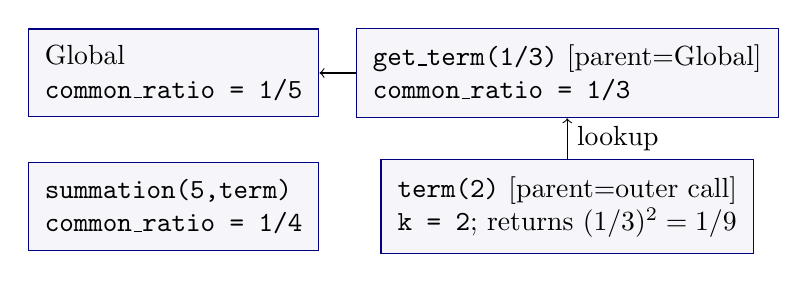
\begin{tikzpicture}[box/.style={draw=NavyBlue,fill=NavyBlue!4,align=left,inner sep=6pt},every node/.style={font=\normalsize}]
\node[box] (global) at (0,0) {Global\\\py{common\_ratio = 1/5}};
\node[box] (outer) at (5,0) {\py{get\_term(1/3)} [parent=Global]\\\py{common\_ratio = 1/3}};
\node[box] (call) at (5,-1.7) {\py{term(2)} [parent=outer call]\\\py{k = 2}; returns $(1/3)^2=1/9$};
\draw[->] (call.north) -- node[right]{lookup} (outer.south);
\draw[->] (outer.west) -- (global.east);
\node[box] at (0,-1.7) {\py{summation(5,term)}\\\py{common\_ratio = 1/4}};
\end{tikzpicture}
\figcap{The returned term's parent is the retained get\_term call. The summation caller's local ratio is outside its lookup chain.}
\end{fig}
\par\noindent\begin{minipage}{\linewidth}
\begin{steps}
\ii The argument $1/3$ is bound to the parameter in the \py{get\_term} frame. The new \py{term} function stores that frame as parent and is returned.
\ii Each later \py{term(k)} finds \py{k} locally and \py{common\_ratio} in that parent frame. The global rebindings do not rebind this parameter.
\ii Thus the five-term sum is $1/3+1/9+1/27+1/81+1/243=121/243$, displayed as approximately $0.4979423868312757$.
\end{steps}
\end{minipage}\par
\textbf{Different actual demo, different parent.} Lecture 6 slide 7 instead creates \py{term=lambda x:pow(common\_ratio,x)} directly in Global. Its later calls find the current global $1/5$, not the old $1/2$ and not the caller's $1/4$. Its five-term sum is $781/3125=0.24992$. Closures retain access to bindings; they do not freeze every value visible when created.

\method{Currying supplies one argument at a time --- Lecture 6, slide 8 and 06.py.}
To convert \py{f(x,y)} into \py{curry(f)(x)(y)}, each returned function must retain the earlier arguments:
\codeblock{curry}
\begin{fig}
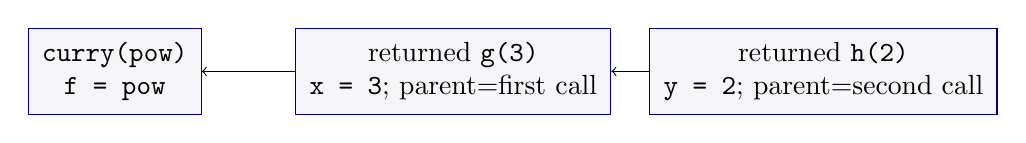
\begin{tikzpicture}[box/.style={draw=NavyBlue,fill=NavyBlue!4,align=center,inner sep=5pt}]
\node[box] (a) at (0,0) {\py{curry(pow)}\\\py{f = pow}};
\node[box] (b) at (4.3,0) {returned \py{g(3)}\\\py{x = 3}; parent=first call};
\node[box] (c) at (9,0) {returned \py{h(2)}\\\py{y = 2}; parent=second call};
\draw[->] (c.west)--(b.east);
\draw[->] (b.west)--(a.east);
\end{tikzpicture}
\figcap{The final body finds $y=2$, then $x=3$, then f=pow, and returns $3^2=9$. Each argument arrives in its own call.}
\end{fig}
Consequently \py{curry(pow)(1/2)(5)=1/32}. In 06.py, \py{summation(5,curry(pow)(3))} supplies the function $k\mapsto3^k$, giving $3+9+27+81+243=363$.

\method{Separate local parameter names from global names.}
Lecture 7 reproduces Fall 2022 MT 1Q1(b): \py{bear=-1; oski=lambda print:print(bear); bear=-2; print(oski(abs))}. The parameter named \py{print} receives \py{abs}; its body finds global \py{bear=-2}, so the inner call returns $2$ without printing. The outer built-in print displays $2$ and returns \py{None}.

\begin{shortcuts}
\ii Lecture 7's small call demo \py{def f(x): y=2; return x+y} gives 6 at x = 4: parameter x and local y belong to that new call.
\ii Write the function's parent when it is created. When called later, copy that parent onto the new call frame; never choose it from the current caller.
\ii The original Lab 2 review's \py{multiply\_by(m)} returns a nested \py{multiply(n)} computing \py{n*m}. After \py{multiply\_by(3)}, global \py{multiply(4)} raises \py{NameError}; retain the returned value or call it immediately.
\ii \py{bool} converts a value's truth to \py{True}/\py{False}. Lecture 7: $0,0.0,\py{''},\py{False}$ are false; $-1$ and \py{' '} are true. \py{bool(print('fool'))} prints \py{fool}, then returns \py{False} because print returns \py{None}.
\end{shortcuts}
\begin{trapbox}
\ii Rebinding a function name does not edit existing references to that function. In Lab 2, \py{more\_cake=cake} retains the function even after \py{cake='cake'}.
\ii A returned function's local name need not exist globally. Returning it preserves the function value and its defining environment, not a new global binding for its inner name.
\end{trapbox}

\section{Trace a rebinding that changes the next iteration}
\begin{qbox}
Why does the following attempt to find a largest input fail on its second iteration, before the loop reaches $10$?
\end{qbox}
Lecture 7 slides 10--11 reproduce a Fall 2022 MT 1Q2 example. The function is:
\par\noindent\begin{minipage}{\linewidth}\lstinputlisting{max_bug.txt}\end{minipage}\par
Run this example in a fresh namespace. The first call \py{f(1)} computes local $y=\max(1,3)=3$ and returns \py{zero}. Its argument \py{lambda z:z-y+10} has Global as parent.
\begin{center}\begin{tabular}{c|l|l}
step&value or action&reason\\\hline
\py{f(1)}&local \py{x=1,y=3}; return \py{zero}&built-in max is still available\\
\py{zero(t)}&\py{t(1)=1-1+10=10}; return $3$&lambda reads global $y=1$\\
first \py{if}&global \py{max=1}; then \py{y=2}&$3$ is true\\
\py{f(2)}&tries \py{1(4,6)}; \py{TypeError}&global max now names an integer
\end{tabular}\end{center}
\par\noindent\begin{minipage}{\linewidth}
\begin{steps}
\ii Local \py{y=3} belongs to the retained \py{f(1)} frame. It is the value returned by \py{zero}, not the global loop variable.
\ii The lambda was created in Global, so its \py{y} is the loop's current $1$. The caller \py{zero}'s parent frame does not become the lambda's parent.
\ii Assignment \py{max=y} changes what later global lookup finds. Rename this result variable to \py{largest} to preserve the built-in function. In the repaired loop all inputs 1--9 pass, so \py{largest=9} and final global \py{y=10}.
\end{steps}
\end{minipage}\par
\begin{shortcuts}
\ii Annotate both a function value and its parent; annotating only its current name loses information when aliases are rebound.
\ii To diagnose a loop, run one complete iteration on paper, update global bindings, then reevaluate the next operator. A successful first iteration does not establish the next call's validity.
\end{shortcuts}
\begin{trapbox}
\ii The local \py{y} in \py{f} does not replace global \py{y}. The actual failure comes from global \py{max}, not from a local integer being returned.
\ii A return ends its call immediately. In Discussion 2's \py{which}, neither the second return nor the assignment after the outer return runs.
\end{trapbox}

\section{Derive searches from the order of the candidates}
\begin{qbox}
For $n=21$, both $19$ and $23$ are prime and equally close. How can a loop guarantee it returns $23$? For digit tests, how can it check every digit without text conversion?
\end{qbox}
A \textbf{prime} is an integer at least 2 with exactly two positive divisors,1 and itself. A \textbf{predicate} returns a Boolean. To count or test candidates, specify which candidates have already been inspected before writing the update.

\textbf{Nearest-prime contract (Lecture 7).} Given an integer $n>5$, return its closest prime; if two primes are equally close, return the greater one.
\begin{motive}
\ii[Want.] Return a closest prime, choosing the greater prime in a tie.
\ii[Know.] At distance $d>0$, the only two candidates are $n+d$ and $n-d$.
\ii[Key step.] Try $n,n+1,n-1,n+2,n-2,\ldots$. Increasing distance establishes closeness; testing the positive offset first establishes the tie rule.
\end{motive}
On positive integers, the supplied \py{is\_prime} helper rejects 1, then tests possible divisors 2 through $n-1$. One divisor disproves primality; exhausting these possibilities proves it by the definition.
\codeblock{nearest}
This is Lecture 7's slight variant of Fall 2022 MT 1Q3(b), using the supplied primality test. In the given template the three fills are \py{is\_prime(n+k)}, \py{n+k}, and \py{-k+1}.
\begin{fig}
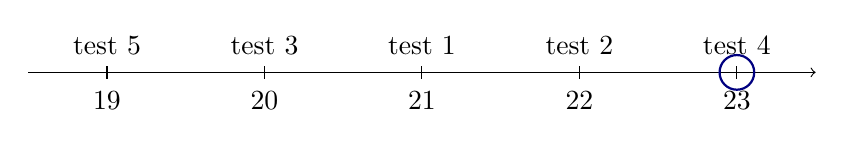
\begin{tikzpicture}
\draw[->] (0,0)--(10,0);
\foreach \x/\v/\a in {1/19/5,3/20/3,5/21/1,7/22/2,9/23/4}{
\draw (\x,.08)--(\x,-.08);
\node[below] at (\x,-.12) {$\v$};\node[above] at (\x,.1) {test \a};}
\draw[NavyBlue,thick] (9,0) circle (.22);
\end{tikzpicture}
\figcap{For 21, test 21,22,20,23. The first prime is 23; equally distant 19 would be tested next.}
\end{fig}
\par\noindent\begin{minipage}{\linewidth}
\begin{steps}
\ii Offset 0 changes to 1. A positive offset $d$ changes to $-d$, then a nonpositive offset $-d$ changes to $d+1$. This generates precisely the required order.
\ii Every smaller distance has failed when the loop returns. At the same positive distance the larger candidate was tested first, proving the tie rule. Thus 8 gives 7,11 gives 11, and 21 gives 23.
\ii For $n>5$, a prime is encountered while $n+k\ge2$: there is a prime 2 or 3 at distance strictly less than $n-2$. The search reaches one of these or an earlier prime. It does not need an unbounded negative-domain primality assumption.
\end{steps}
\end{minipage}\par

\method{Use the same scan with a different decision --- Lab 2 and Discussion 2.}
For integers 1 through $n$, keep an index \py{i} and inspect it once. Lab 2's \py{count\_cond(condition)} retains a two-argument predicate; its returned function counts those indices with \py{condition(n,i)} true. Discussion 2's \py{make\_keeper(n)} retains the bound instead; its returned function receives the predicate and prints the matching indices. The changing quantities are the same; which argument arrives first determines which frame retains it.

For a positive integer $x$, \py{x\%10} is the last digit and \py{x//10} removes it. Integer division by $10^{k-1}$ first removes the $k-1$ digits to the right; a final remainder extracts the $k$th digit. This proves Discussion 2's \py{find\_digit(k)} formula. Missing digits give 0 because the quotient is 0.
\begin{fig}
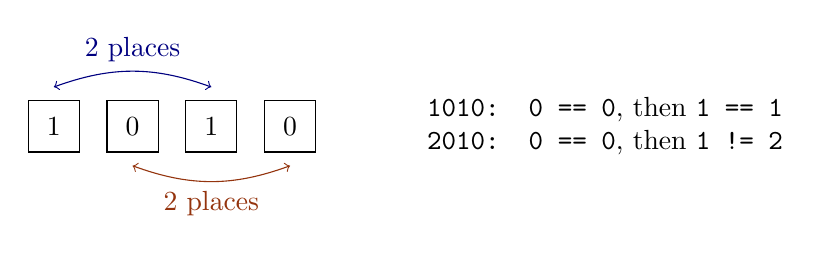
\begin{tikzpicture}[every node/.style={font=\normalsize}]
\foreach \x/\d in {0/1,1/0,2/1,3/0}{\node[draw,minimum size=.65cm] at (\x,0) {$\d$};}
\draw[<->,NavyBlue] (0,.5) to[bend left=20] node[above] {2 places} (2,.5);
\draw[<->,RawSienna] (1,-.5) to[bend right=20] node[below] {2 places} (3,-.5);
\node[align=left] at (7,0) {\py{1010: 0 == 0}, then \py{1 == 1}\\\py{2010: 0 == 0}, then \py{1 != 2}};
\end{tikzpicture}
\figcap{Match\_k compares only digit pairs that both exist. For k=2 the two pairs of 1010 agree; the second pair of 2010 fails.}
\end{fig}
\par\noindent\begin{minipage}{\linewidth}
\begin{steps}
\ii To compare digits $k$ places apart, compare \py{x\%10} with \py{(x//10**k)\%10}, then remove one digit. Continue only while \py{x//10**k > 0}, so both compared digits exist.
\ii One unequal pair disproves the universal claim and returns \py{False}. If all pairs were removed without a failure, return \py{True}. A number with at most $k$ digits has no such pair and therefore passes.
\ii The same argument gives \py{every(t)}: one failing digit returns false; reaching the end proves all passed. \py{count\_if(f)} instead increments a count for each passing digit. These are different final questions on the same right-to-left scan.
\end{steps}
\end{minipage}\par
\begin{shortcuts}
\ii A reusable returned function needs a fresh counter and working input inside each call. Moving an integer counter outside while retaining a local increment would instead leave that local name uninitialized; keep the initialization with its loop.
\ii For Lab 2's cycle, the number of applications already done has remainders $0,1,2,0,\ldots$ modulo 3. Select \py{f1,f2,f3} accordingly; zero applications returns the original input.
\end{shortcuts}
\begin{trapbox}
\ii A first matching digit is insufficient for \py{every}. For an odd-digit test,37511 passes but 2023 fails despite its last digit 3 passing.
\ii \py{match\_k(1)(1)} is true because there are no pairs; comparing a nonexistent left digit to 0 would reject it incorrectly. Use positive $k$ and positive input; a negative $k$ is outside the arithmetic scan's intended domain.
\ii In \py{count\_cond}, pass \emph{both} \py{n,i} to the predicate. Counting multiples with digit sum 5 tests \py{sum\_digits(n*i)}, not merely \py{sum\_digits(i)}.
\end{trapbox}

\section{Problem set}
\begin{prob}
\textbf{Lab 2 Q1: The Truth Will Prevail.} Predict every prompt display, including output effects, returned strings and errors. The session continues after an error. These are the original lab inputs; each blank is an output line.
\lstinputlisting{short_circuit.txt}
\hint{Use the short-circuit rule; only not must return a Boolean.}
\end{prob}
\begin{prob}
\textbf{Lab 2 Q2: Higher-Order Functions.} Trace the following session. Write FUNCTION for a function value and distinguish the printed lines from returned values.
\lstinputlisting{hof_wwpd.txt}
\hint{Follow the current global bindings of cake, more\_cake and chocolate at each call.}
\end{prob}
\begin{prob}
\textbf{Lab 2 Q3: Lambda.} Predict each display in this original session. A bare None value produces no display at the interactive prompt.
\lstinputlisting{lambda_wwpd.txt}
\hint{Creating a lambda does not execute its expression; count how many argument lists are supplied.}
\end{prob}
\begin{prob}
\textbf{Lab 2 Q4: Piecewise.} Return a one-argument function using \py{f(x)} for $x<b$ and \py{g(x)} otherwise. With negate, identity and $b=0$, inputs 6 and $-1$ give 6 and 1.\par
\hint{Retain f,g,b in the defining frame; make the choice inside the returned function.}
\end{prob}
\begin{prob}
\textbf{Lab 2 Q5: Count Cond.} Return a one-argument function counting indices $1\le i\le n$ with \py{condition(n,i)} true. Use it to recover \py{count\_fives}, where \py{sum\_digits(n*i)==5}, and \py{count\_primes}, where \py{is\_prime(i)}. Provided sum\_digits accepts nonnegative integers; provided is\_prime accepts positive integers. Source checks: fives at 10/50 give 1/4; primes at 2/3/4/5/20 give 1/2/2/3/8. The source's initial direct loops also give \py{count\_primes(6)=3} and \py{count\_primes(13)=6}.\par
\hint{Keep the index and count inside each call of the returned function.}
\end{prob}
\begin{prob}
\textbf{Lab 2 Q6: HOF Diagram Practice.} Draw all frames, values, parent links and function objects after this code. There is no submitted code for this question.
\codeblock{lab_diagram}
\hint{Evaluate the right side of f=f(g,n) using the old f; then evaluate g's right side before rebinding g.}
\end{prob}
\begin{prob}
\textbf{Lab 2 Q7: Week 3 Survey.} The assignment asks you to complete the \href{https://forms.gle/nbhRwerW4MQEWWDB8}{official Week 3 Survey} and place its completion passphrase in the starter's \py{passphrase} string. The form is now closed; its questions and completion passphrase are unavailable here.\par
\hint{This is a personal administrative submission; the worksheet supplies no answer or passphrase.}
\end{prob}
\begin{prob}
\textbf{Lab 2 Q8 (optional): I Heard You Liked Functions.} Implement \py{cycle(f1,f2,f3)} returning \py{g(n)}, which returns \py{h(x)} applying exactly $n\ge0$ functions in cyclic order f1,f2,f3,f1,\ldots. With add1, times2, add3, source checks are $n,x$: $(0,5)\mapsto5$, $(2,1)\mapsto4$, $(3,2)\mapsto9$, $(4,2)\mapsto10$, $(6,1)\mapsto19$.\par
\hint{Use the application counter modulo 3 to choose the next function.}
\end{prob}

Use \py{python3 -m pytest -k piecewise} for the corresponding code test; replace the final name with \py{count\_cond}, \py{cycle} or \py{week3\_survey} as appropriate. For the three WWPD groups use \py{short\_circuit}, \py{hof\_wwpd}, or \py{lambda\_wwpd} with \py{--unlock}. WWPD responses are not submitted. Prepare the submission bundle with the Provenance command in VS Code and upload its zip to Gradescope.

\subsection{Discussion 2}
\begin{prob}
\textbf{Q1: Warm Up.} Find \py{result=(lambda x:2*(lambda x:3)(4)*x)(5)}.\par
\hint{The inner and outer x belong to different calls.}
\end{prob}
\begin{prob}
\textbf{Q2: Teamwork.} Draw the complete environment diagram and determine the final global bindings.
\codeblock{teamwork}
\hint{The call to team reads global t=abs; the dream call's local t is separate.}
\end{prob}
\begin{prob}
\textbf{Q3: Make Keeper.} For positive integer $n$, return a function taking cond and printing each integer 1 through $n$ with \py{cond(i)} true, one per line. Source tests at $n=5$: even test prints 2,4; always-true prints 1--5; always-false prints nothing.\par
\hint{Choose which argument is retained before the scanning function is returned.}
\end{prob}
\begin{prob}
\textbf{Q4: Digit Finder.} For positive integer $k$, return a function giving the $k$th digit from the right of positive integer $x$, or 0 if absent. Retain the given \py{assert k>0}; use a single lambda return expression, no strings or indexing. Source checks $(k,x)=(2,3456),(2,5678),(1,10),(4,789)$ give 5,7,0,0.\par
\hint{Remove k-1 rightmost digits, then take remainder 10.}
\end{prob}
\begin{prob}
\textbf{Q5: Match Maker.} Return \py{check(x)} testing whether every pair of digits $k$ places apart agrees. Use positive integer $k,x$; no strings/indexing; find\_digit is allowed. Source true cases: $(2,1010),(1,1),(3,123123)$; false: $(2,2010),(1,1010),(1,2111111111111111),(2,123123)$. Fill the source template:
\begin{lstlisting}
def match_k(k):
    def check(x):
        while x // (10**k) > 0:
            if ____________________:
                return ____________
            x //= 10
        ___________________________
    _______________________________
\end{lstlisting}
\hint{Compare only pairs with both digits present; one failure is decisive.}
\end{prob}
\begin{prob}
\textbf{Q6 (optional; Spring 2024 MT 1Q1(b)): Which One.} What does \py{which()()} display?
\codeblock{which}
\hint{Follow the stored parent and stop at each executed return.}
\end{prob}
\begin{prob}
\textbf{Q7 (optional; Fall 2023 MT 1Q4(b)): Choose Wisely.} A digit test takes an integer 0--9 and returns a Boolean. Return a function that tests whether it is true for every digit of a positive integer. The original last two blanks were multiple choice; here fill the worksheet's blanks:
\begin{lstlisting}
def every(t):
    def digit(n):
        assert n > 0
        while n:
            if ____________________:
                ___________________
            n = n // 10
        return ____________________
    return ________________________
\end{lstlisting}
Source tests: odd-digit predicate gives true for 37511, false for 2023.\par
\hint{Return false on the first failing digit; reaching zero proves every digit passed.}
\end{prob}
\begin{prob}
\textbf{Q8 (optional; Spring 2024 MT 1Q4(b,c)): Nice Dice.} Fill the count\_if predicate and count\_at\_least argument. The latter blank was multiple choice on the exam. Input $n$ is positive; threshold $k$ is positive.
\begin{lstlisting}
def count_if(f):
    def g(n):
        count = 0
        while n:
            if ____________________:
                count += 1
            n = n // 10
        return count
    return g

def count_at_least(k):
    return count_if(_______________)
\end{lstlisting}
For 431663334231, count of 3s is 5 and count of digits at least 3 is 9.\par
\hint{Supply a digit predicate to reuse the existing scan.}
\end{prob}

\subsection{Actual exam practice}
\begin{prob}
\textbf{Fall 2022 MT 1Q4(a), reproduced in Lecture 6 slide 13.} Choose all implementations of funsquare that take one argument f and return a one-argument function computing \py{f(f(x))}. The original example defines \py{triple=lambda x:3*x} and requires \py{funsquare(triple)(5)=45}. The option suffixes below merely distinguish the six separate original alternatives; each was originally named funsquare.
\codeblock{funsquare}
\hint{Check both signatures before testing triple(5); defer both calls to f until x arrives.}
\end{prob}
\begin{prob}
\textbf{Fall 2026 MT 1Q2: New Print, p3.} Write every printed line. Run this source code in its own namespace; the display is the same in a file or at the prompt.
\codeblock{new_print}
\begin{lstlisting}
og = print
print = new_print(print)
print = new_print(print)
og('print returned', print(2))
\end{lstlisting}
\hint{Name the original print P0 and the two returned functions P1,P2. Record each function's retained print separately.}
\end{prob}
\begin{prob}
\textbf{Fall 2026 MT 1Q4.3: Make Gap, p6 (optional zero-point A+ question).} Use the supplied gap and f helpers. The returned function takes $n$ and term, selects those indices 1 through $n$ with \py{use(i)} true, and returns the largest absolute difference between consecutive selected term values. Assume at least two indices pass and use gives a stable truth result at each index on repeated calls.
\codeblock{gap_tool}
\begin{lstlisting}
def f(use, go, then):
    y, i = 0, 0
    while go(y, i):
        i += 1
        if use(i):
            y += 1
    return then(y, i)

def make_gap(use):
    return lambda n, term: gap(__________)
\end{lstlisting}
No \py{for, :=, [, ], if, else, and, or, map, filter, range} in your answer. Source example: odd indices with $n=8$, \py{term=lambda x:x\%5}, give 1,3,0,2 and result 3.\par
\hint{Call f once to count selected indices, then use another call to locate the jth selected index.}
\end{prob}
\textbf{Continuing assignments.} HW 2 is due September 10, Hog Phase 1 through P5 September 10, full Hog September 17. Their complete statements and solutions are in Week 2; no new homework is assigned this week. Lab 2 is due September 9 at 11:59p.m. Quiz 1 Functions is listed September 8, but no public question sheet is linked.

\textbf{Attribution.} Official Fall 2026 CS 61A lectures, labs, discussions and saved real exams; lecture-reproduced earlier exams are identified above. The supplied code is preserved in the source cache. Exact coverage, execution checks and source limitations are recorded in audit.md.

\end{document}
